\documentclass[conference]{IEEEtran}
\IEEEoverridecommandlockouts

% --- Standard IEEE Packages ---
\usepackage{cite}
\usepackage{amsmath,amssymb,amsfonts}
\usepackage{algorithmic}
\usepackage{graphicx}
\usepackage{textcomp}
\usepackage{xcolor}
\usepackage{booktabs}
\usepackage{url}
\usepackage{subcaption}

\def\BibTeX{{\rm B\kern-.05em{\sc i\kern-.025em b}\kern-.08em
    T\kern-.1667em\lower.7ex\hbox{E}\kern-.125emX}}

\begin{document}

\title{A Priority-Aware Fog-Assisted Framework for Real-Time Clinical Monitoring in Healthcare IoT\\
\thanks{This research was conducted as part of the Cloud Computing undergraduate curriculum (Topic 19) at the Indian Institute of Information Technology (IIIT) Sri City, India. All experimental artifacts and simulation code are open-source and reproducible.}
}

\author{
\IEEEauthorblockN{A. Krishna\IEEEauthorrefmark{1}, Student Co-Author II\IEEEauthorrefmark{2}, and Student Co-Author III\IEEEauthorrefmark{3}}
\IEEEauthorblockA{Department of Computer Science and Engineering\\
Indian Institute of Information Technology (IIIT) Sri City, Chittoor, Andhra Pradesh, India\\
Email: \IEEEauthorrefmark{1}krishna.a@iiits.in, \IEEEauthorrefmark{2}student2@iiits.in, \IEEEauthorrefmark{3}student3@iiits.in}
}

\maketitle

\begin{abstract}
Continuous physiological telemetry in connected healthcare—monitoring heart rate, oxygen saturation ($\text{SpO}_2$), body temperature, and blood pressure—generates massive streams of time-series data. Transmitting raw biometric readings directly across Wide Area Networks (WAN) to centralized cloud datacenters incurs high transit latency, severe packet jitter, and excessive bandwidth consumption, jeopardizing patient safety during acute hemodynamic crises. While fog computing addresses WAN bottlenecks by relocating computation to local network gateways, conventional edge filtering and window-based aggregation inadvertently introduce a dangerous clinical safety hazard: time-critical physiological alarms queue behind routine biometric readings in First-In-First-Out (FIFO) aggregation buffers, creating a lethal ``latency cliff.''

In this paper, we propose and evaluate an end-to-end, priority-aware fog-assisted healthcare monitoring architecture modeled and simulated in iFogSim2. Our framework couples stateful delta-filtering and sliding-window aggregation for routine vital signs with a dedicated, zero-buffering local emergency bypass channel for life-critical anomalies. Through four rigorously controlled experiments comprising 44,000 synthetic clinical readings across 10 to 50 patients (40 to 200 sensors), we contrast four paradigms: Cloud-Only Baseline (A), Fog Forwarding (B), Naive Fog Filtering and Aggregation (C), and Priority-Aware Fog (D). Empirical results demonstrate that while naive edge aggregation (C) yields a 77.22\% cloud bandwidth saving, it imposes a 2,293.52\,ms critical alert delay, causing Service Level Agreement (SLA $\le$ 500\,ms) compliance to crash to 27.88\%. In contrast, our proposed architecture (D) decouples critical response from aggregation window size ($W$), achieving an emergency alert latency of 7.13\,ms (a 96.57\% reduction over Cloud-Only), conserving 66.62\% to 79.64\% of cloud bandwidth, and maintaining 100.00\% clinical SLA reliability even under severe WAN bottlenecks and rural network degradation.
\end{abstract}

\begin{IEEEkeywords}
Fog computing, Healthcare IoT, iFogSim2, real-time vital monitoring, delta-filtering, sliding-window aggregation, priority bypass, quality of service (QoS).
\end{IEEEkeywords}

% ========================================================================
% SECTION I: INTRODUCTION
% ========================================================================
\section{Introduction}
The rapid proliferation of wearable and bedside Internet-of-Things (IoT) medical devices has catalyzed real-time physiological telemetry in intensive care units (ICUs), post-operative wards, and ambulatory smart homes. Modern clinical protocols require continuous, multi-parameter vital sign monitoring, including Heart Rate (HR), Blood Oxygen Saturation ($\text{SpO}_2$), Core Body Temperature (TEMP), and Systolic/Diastolic Blood Pressure (BP). When sampled at high frequencies across dozens of monitored beds, these biosensors emit relentless streams of discrete measurement tuples.

Historically, Internet of Medical Things (IoMT) systems have adopted a \textit{Cloud-Only} architecture, wherein raw sensor tuples traverse local access bridges, hospital border routers, and multi-hop Wide Area Network (WAN) backhauls to reach hyper-scale cloud datacenters for centralized analytics, alerting, and Electronic Health Record (EHR) ingestion~\cite{Gupta2017,Kraemer2017}. However, routing high-frequency physiological streams exclusively to the cloud exposes two fundamental architectural limitations:
\begin{enumerate}
    \item \textbf{WAN Latency and Network Jitter:} Uncontrolled wide-area round-trip times (RTT $\ge 200$\,ms) and transit jitter prevent cloud analytics from honoring the strict sub-second response times ($\le 500$\,ms) mandated by medical standards for acute hemodynamic crises (e.g., ventricular tachycardia, acute hypoxemia, or malignant hypertensive crisis)~\cite{Kraemer2017,Verma2018}.
    \item \textbf{Bandwidth and Ingress Explosion:} Up to 85\% of physiological readings captured from stable patients represent redundant, clinically stationary measurements (e.g., resting heart rate fluctuating by $< 1$\,bpm). Streaming uncompressed, raw telemetry continuously across the WAN saturates backhaul bandwidth and generates massive cloud storage ingestion overhead~\cite{Aazam2014,Pace2019}.
\end{enumerate}

To mitigate these drawbacks, \textit{Fog Computing} has emerged as an intermediate architectural tier that situates computation, storage, and networking resources at the edge of the local network, such as hospital ward gateways or bedside micro-servers~\cite{Mahmud2022,Rahmani2018}. By performing data cleaning, duplicate suppression, and windowed aggregation at the fog tier, WAN traffic can be cut by more than 70\%~\cite{Pace2019,Aazam2014}.

Nevertheless, a critical research gap persists in contemporary edge healthcare literature. Conventional edge aggregation architectures aggregate incoming telemetry tuples into sliding or tumbling batch windows ($W$) before WAN transmission~\cite{Pace2019}. While effective for stationary signals, uniform FIFO window buffering introduces a devastating clinical side-effect: \textit{The Aggregation Latency Cliff}. When an acute cardiac arrest or oxygen desaturation event occurs, the critical tuple is enqueued behind routine readings inside the edge buffer, remaining stalled until the entire window fills. Under typical telemetry sampling rates, this introduces multi-second delays, directly violating medical SLAs and creating an unacceptable clinical hazard.

\subsection{Research Contributions}
To resolve this fundamental tension between WAN bandwidth conservation and clinical emergency responsiveness, this paper presents a comprehensive, reproducible investigation into fog-assisted healthcare architectures using the discrete-event simulator iFogSim2~\cite{Mahmud2022}. Our key contributions are:
\begin{itemize}
    \item \textbf{Decoupled Multi-Tier Architecture:} We design and implement four comparative healthcare paradigms: Cloud-Only Baseline (A), Fog Forwarding (B), Naive Fog Filtering and Aggregation (C), and Priority-Aware Fog with Local Emergency Bypass (D).
    \item \textbf{Algorithmic Formulation:} We formulate a lightweight, stateful delta-filtering algorithm ($\Delta_{\text{thresh}}$) coupled with sliding-window aggregation ($W$) for normal streams, and a three-tier clinical triage engine ($\text{NORMAL}$, $\text{ABNORMAL}$, $\text{CRITICAL}$) that bifurcates the data plane. Critical alarms bypass aggregation buffers and WAN links completely, executing closed-loop actuation over the local hospital LAN in 7.13\,ms while asynchronously archiving to the cloud.
    \item \textbf{Rigorous Empirical Benchmarking:} Using a fully deterministic synthetic workload (44,000 readings across $10$ to $50$ patients), we conduct four controlled parameter sweeps evaluating architectural baseline overhead, patient scalability up to 200 sensors, aggregation window sensitivity ($W \in \{1, 2, 5, 10, 20\}$), and WAN degradation profiles (down to 100\,Kbps, 600\,ms WAN).
    \item \textbf{Open-Source Reproducibility:} All simulation code, experimental harness scripts, CSV raw traces, and Python visualization pipelines are publicly documented to establish a rigorous university research baseline.
\end{itemize}

% ========================================================================
% SECTION II: RELATED WORK
% ========================================================================
\section{Related Work}
The convergence of edge computing and medical telemetry has generated substantial literature over the past decade. We categorize prior work across three primary dimensions: simulation environments, smart e-Health gateways, and edge filtering/routing techniques.

\subsection{Fog Computing Simulation Frameworks}
Evaluating large-scale fog topologies on physical hardware is logistically prohibitive and financially exorbitant. Gupta et al.~\cite{Gupta2017} developed \textit{iFogSim}, an open-source discrete-event simulator built upon CloudSim. iFogSim formalized the modeling of fog infrastructure as physical hierarchies of \texttt{FogDevice} nodes, application modules as Directed Acyclic Graph (\texttt{DAG}) vertices, and network traffic as discrete \texttt{Tuple} entities. Recently, Mahmud et al.~\cite{Mahmud2022} introduced \textit{iFogSim2}, extending the framework with dynamic clustering, microservice orchestration, and mobility management. While iFogSim2 includes canonical healthcare demonstrations (e.g., cardiovascular monitoring), it models uniform data streams without physiological severity classification or stateful delta-compression. Our work builds directly upon iFogSim2, providing custom, production-grade clinical processing classes.

\subsection{Smart e-Health Gateways and Edge Architectures}
The concept of deploying intermediate intelligence near medical sensors was pioneered by Rahmani et al.~\cite{Rahmani2018} through the \textit{UT-GATE} smart e-Health gateway. Deployed on embedded ARM and Linux gateways, UT-GATE validated local protocol bridging, local alerting, and data persistence during WAN network blackouts. Gia et al.~\cite{Gia2015} demonstrated edge-based QRS detection and feature extraction from raw ECG signals, achieving over 90\% bandwidth reduction compared to transmitting raw electrical waveforms. Kraemer et al.~\cite{Kraemer2017} and Mutlag et al.~\cite{Mutlag2019} provided exhaustive taxonomic surveys, establishing that time-sensitive healthcare alerts must be handled near the patient boundary rather than deferred to remote cloud infrastructure. However, these systems were evaluated on small-scale laboratory prototypes (1--3 patients) and lacked systematic stress testing under varying aggregation windows and degraded wide-area networks.

\subsection{Data Filtering, Window Aggregation, and Priority Routing}
Data trimming and duplicate suppression at smart gateways were established by Aazam and Huh~\cite{Aazam2014}, who demonstrated up to 80\% reduction in cloud-bound IoT traffic by filtering stagnant samples. In the medical domain, Pace et al.~\cite{Pace2019} designed BodyCloud, an edge-centric architecture using sliding-window aggregation to extend the battery lifetimes of Body Sensor Networks (BSNs). Verma and Sood~\cite{Verma2018} implemented rule-based edge processing in smart home health monitoring, reducing average latency from 1,850\,ms to 290\,ms. Tuli et al.~\cite{Tuli2020} developed \textit{HealthFog}, deploying deep learning ensembles across edge nodes for cardiac diagnosis. Nevertheless, none of these works explicitly analyzed the structural \textit{latency cliff} introduced when critical medical alarms are co-located in FIFO aggregation buffers alongside routine vitals. Table~\ref{tab:related_work} presents a taxonomic comparison of our architecture against prior art.

\begin{table*}[t]
\centering
\caption{Taxonomic Comparison of Related Literature in Edge/Fog Healthcare Monitoring}
\label{tab:related_work}
\begin{tabular}{lcccccc}
\toprule
\textbf{Publication} & \textbf{Environment} & \textbf{Vital Modalities} & \textbf{Edge Delta-Filtering} & \textbf{Window Aggregation} & \textbf{Priority LAN Bypass} & \textbf{Strict SLA Tracking} \\
\midrule
Gupta et al.~\cite{Gupta2017} & iFogSim & Generic / EEG & No & No & No & No \\
Mahmud et al.~\cite{Mahmud2022} & iFogSim2 & Generic Microservices & No & No & No & No \\
Rahmani et al.~\cite{Rahmani2018} & UT-GATE Lab & ECG, Temp & Basic Threshold & No & Partial & No \\
Gia et al.~\cite{Gia2015} & Hardware Testbed & ECG (QRS) & Feature Extraction & No & No & No \\
Kraemer et al.~\cite{Kraemer2017} & Survey / Review & Multi-Parameter & Conceptual & No & Conceptual & No \\
Mutlag et al.~\cite{Mutlag2019} & Survey / Taxonomy & Multi-Parameter & No & No & Conceptual & No \\
Verma \& Sood~\cite{Verma2018} & Simulation & Multi-Vital & Rule-based & No & No & No \\
Tuli et al.~\cite{Tuli2020} & FogBus / iFogSim & Cardiovascular & No & No & No & Partial \\
Pace et al.~\cite{Pace2019} & BodyCloud & Generic BSN & Threshold & Yes ($W$) & No & No \\
Aazam \& Huh~\cite{Aazam2014} & FiCloud Testbed & Generic IoT & Trimming & No & No & No \\
\midrule
\textbf{Our Framework (Topic 19)} & \textbf{iFogSim2} & \textbf{HR, $\text{SpO}_2$, TEMP, BP} & \textbf{Stateful ($\Delta_{\text{thresh}}$)} & \textbf{Configurable ($W$)} & \textbf{Dedicated Local Path} & \textbf{Strict ($\le$ 500\,ms)} \\
\bottomrule
\end{tabular}
\end{table*}

% ========================================================================
% SECTION III: SYSTEM ARCHITECTURE & METHODOLOGY
% ========================================================================
\section{System Architecture and Methodology}
We formulate a hierarchical, three-tier cyber-physical topology consisting of: (1) Patient IoT Sensor Tier, (2) Hospital Ward Fog Gateway Tier, and (3) Cloud Datacenter Tier. Fig.~\ref{fig:arch_diagram} illustrates the overall system architecture and data plane bifurcation.

\begin{figure}[b]
\centering
\fbox{\parbox{0.95\columnwidth}{\centering\footnotesize
\textbf{[Patient Bedside IoT Sensors]}\\[-2pt]
Heart Rate, $\text{SpO}_2$, Body Temp, Blood Pressure (Period = 1,000\,ms)\\[2pt]
$\Big\downarrow$ Local LAN ($2.0$\,ms, 10\,Gbps)\\[2pt]
\textbf{[Hospital Ward Fog Gateway]}\\[-2pt]
Stateful Delta-Filter ($\Delta_{\text{thresh}}$) $\longrightarrow$ \textit{Suppresses Redundant Normal Vitals}\\[2pt]
Three-Tier Priority Classifier:\\
$\bullet$ \textbf{CRITICAL} $\Longrightarrow$ \textbf{Local Emergency Bypass} $\xrightarrow{\text{LAN (1.0\,ms)}}$ \textbf{[Bedside Alarm Actuator]}\\[-1pt]
$\quad\quad\quad\quad\quad\quad\quad\quad\quad\quad\quad\quad\quad\quad\quad\quad\quad\searrow$ Asynchronous Copy to Cloud EHR\\
$\bullet$ \textbf{ABNORMAL} $\Longrightarrow$ Direct WAN Dispatch (No Window Wait)\\[-1pt]
$\bullet$ \textbf{NORMAL} $\Longrightarrow$ Sliding-Window Aggregation ($W$ readings per tuple)\\[2pt]
$\Big\downarrow$ Wide Area Network (WAN: 100\,ms, 100\,Mbps nominal)\\[2pt]
\textbf{[Cloud Datacenter Tier]}\\[-2pt]
Long-Term Analytics, Medical History Storage, EHR Auditing
}}
\caption{Three-tier healthcare IoT topology with data-plane priority bifurcation.}
\label{fig:arch_diagram}
\end{figure}

\subsection{Physical Topology and Network Modeling}
Let $\mathcal{P} = \{P_1, P_2, \dots, P_N\}$ denote the set of $N$ monitored patients in a hospital ward. Each patient $P_i$ is instrumented with four biomedical sensors:
$$\mathcal{S}_i = \{S_{i}^{\text{HR}}, S_{i}^{\text{SpO}_2}, S_{i}^{\text{TEMP}}, S_{i}^{\text{BP}}\}$$
yielding total sensor population $|\mathcal{S}| = 4N$. Each sensor generates synthetic physiological tuples of size $L_{\text{sensor}} = 500$\,Bytes at fixed interval $\Delta t_{\text{sample}} = 1{,}000$\,ms.

The bedside sensors connect to a ward-level intermediate computing node, the \textit{Hospital Fog Gateway}, via a dedicated switched Ethernet/WLAN connection with propagation delay $d_{\text{LAN}} = 2.0$\,ms and bandwidth $B_{\text{LAN}} = 10{,}000$\,Mbps (10\,Gbps). The fog gateway is an 8-core edge server provisioned with 8,000\,MIPS processing capacity and 8,000\,MB RAM.

The fog gateway connects to the centralized \textit{Cloud Datacenter} across a dedicated WAN link characterized by propagation delay $d_{\text{WAN}}$ (nominally 100\,ms) and uplink bandwidth $B_{\text{WAN}}$ (nominally 100\,Mbps). The cloud datacenter is modeled as an enterprise multi-processor cluster equipped with 44,000\,MIPS and 40,000\,MB RAM. Finally, each patient bed features a bedside actuator (visual monitor/alarm bell) linked to the fog gateway with delay $d_{\text{act}} = 1.0$\,ms.

\subsection{Architectural Taxonomy (Architectures A--D)}
To rigorously evaluate the isolated impact of each edge mechanism, we implement four mutually exclusive architectures:

\begin{enumerate}
    \item \textbf{Architecture A (Cloud-Only Baseline):} Medical sensors transmit all raw readings across the WAN directly to the cloud. The cloud executes analytics and returns an alarm tuple back across the WAN to the bedside actuator. No edge processing is performed.
    \item \textbf{Architecture B (Fog Forwarding):} Tuples transit through the hospital fog gateway, which executes a passive inspection module (\texttt{fog\_forwarder}, consuming 200\,MIPS) before forwarding 100\% of raw readings to the cloud over WAN. This isolates the pure latency overhead of an intermediate gateway hop.
    \item \textbf{Architecture C (Naive Fog Filtering and Window Aggregation):} The fog gateway hosts a \texttt{fog\_filter\_aggregator} module. It implements delta-filtering and batches tuples into sliding windows of size $W$. Once full, the batch tuple is transmitted over WAN to the cloud, which processes the window and dispatches actuator notifications back over WAN. No priority distinction is made; critical alarms are queued indiscriminately inside the window buffer.
    \item \textbf{Architecture D (Priority-Aware Fog with Local Emergency Bypass):} The fog gateway hosts an intelligent \texttt{priority\_fog\_processor} implementing data plane bifurcation. It classifies every incoming vital into three clinical tiers:
    \begin{itemize}
        \item \textbf{CRITICAL:} Instantly dispatches a lightweight alert tuple ($L_{\text{alert}} = 200$\,Bytes) directly to the local bedside actuator over the LAN ($1.0$\,ms), completely bypassing the WAN and aggregation buffers. Concurrently, an asynchronous copy is transmitted to the cloud for EHR archival.
        \item \textbf{ABNORMAL:} Dispatched immediately over WAN to cloud analytics without window buffering, ensuring prompt clinical review without aggregation delay.
        \item \textbf{NORMAL:} Filtered via stateful delta-suppression ($\Delta_{\text{thresh}}$). Readings that do not change significantly from the last reported state are discarded. Retained normal vitals are batched into windows of size $W$ and forwarded to the cloud in compressed multi-sample tuples ($L_{\text{batch}} = 1{,}200$\,Bytes).
    \end{itemize}
\end{enumerate}

\subsection{Mathematical Formulations}
The end-to-end latency $T_{\text{e2e}}$ of a vital sign tuple is defined as the elapsed time from its generation at sensor $S_{i,j}$ ($t_{\text{gen}}$) to the delivery of the corresponding action tuple at the actuator ($t_{\text{act}}$):
\begin{equation}
T_{\text{e2e}} = t_{\text{act}} - t_{\text{gen}} = T_{\text{prop}} + T_{\text{trans}} + T_{\text{proc}} + T_{\text{queue}} + T_{\text{buf}}
\end{equation}
where $T_{\text{prop}}$ is total propagation delay, $T_{\text{trans}} = \frac{L}{B}$ is transmission delay, $T_{\text{proc}} = \frac{\text{CPU Demand}}{\text{MIPS}}$ is processing time, $T_{\text{queue}}$ is network queueing delay, and $T_{\text{buf}}$ is the buffering delay incurred while waiting for an aggregation window to fill.

For Architecture A, the theoretical minimum round-trip latency across the WAN is:
\begin{equation}
T_{\text{e2e}}^{\text{Arch A}} \approx 2 \times d_{\text{WAN}} + 2 \times d_{\text{LAN}} + T_{\text{proc}}^{\text{cloud}} \approx 200 + 4 + 3.7 \approx 207.7\,\text{ms}
\end{equation}

In Architecture C, an incoming critical vital that enters an empty aggregation window of size $W$ incurs a buffering delay:
\begin{equation}
T_{\text{buf}} = (W - 1) \times \Delta t_{\text{sample}}
\end{equation}
yielding an expected critical alert latency:
\begin{equation}
T_{\text{e2e}}^{\text{Arch C, Crit}} \approx T_{\text{buf}} + 2 \times d_{\text{WAN}} + T_{\text{proc}}^{\text{fog}} + T_{\text{proc}}^{\text{cloud}} \gg 500\,\text{ms}
\end{equation}

In Architecture D, critical vitals bypass both $T_{\text{buf}}$ and the WAN entirely, traversing only the local switched network:
\begin{equation}
T_{\text{e2e}}^{\text{Arch D, Crit}} = d_{\text{LAN}} + T_{\text{proc}}^{\text{fog}} + d_{\text{act}} = 2.0\,\text{ms} + \frac{200}{8000}\,\text{ms} + 1.0\,\text{ms} \approx 7.13\,\text{ms}
\end{equation}

Cloud Bandwidth Saving ($\text{BWS}_{\text{cloud}}$) relative to the Cloud-Only baseline is formalized as:
\begin{equation}
\text{BWS}_{\text{cloud}} = \left( 1 - \frac{\text{Traffic}_{\text{cloud}}^{\text{arch}}}{\text{Traffic}_{\text{cloud}}^{\text{Arch A}}} \right) \times 100\%
\end{equation}

Finally, for clinical emergency events, Service Level Agreement (SLA) Reliability $\mathcal{R}_{\text{SLA}}$ against the medical deadline $\tau_{\text{SLA}} = 500$\,ms is given by:
\begin{equation}
\mathcal{R}_{\text{SLA}} = \frac{1}{M_{\text{crit}}} \sum_{k=1}^{M_{\text{crit}}} \mathbb{I}(T_{\text{e2e}}^{(k)} \le \tau_{\text{SLA}}) \times 100\%
\end{equation}
where $M_{\text{crit}}$ is the total number of critical tuples generated, and $\mathbb{I}(\cdot)$ is the indicator function.

% ========================================================================
% SECTION IV: EXPERIMENTAL SETUP
% ========================================================================
\section{Experimental Setup in iFogSim2}

\subsection{Physiological Telemetry and Severity Model}
To ensure clinical realism, the synthetic generator simulates vital signs using bounded Gaussian random walks calibrated against human physiological ranges~\cite{Kraemer2017,Verma2018}. Each reading $v(t)$ evolves according to:
\begin{equation}
v(t) = v(t-1) + \mathcal{N}(0, \sigma^2)
\end{equation}
subject to hard clinical physiological boundaries. Table~\ref{tab:clinical_thresholds} enumerates the clinical boundaries, delta-filtering thresholds ($\Delta_{\text{thresh}}$), and empirical distribution across our benchmark workload.

\begin{table}[htbp]
\centering
\caption{Physiological Vital Signs, Clinical Triage Ranges, and Delta-Filtering Thresholds}
\label{tab:clinical_thresholds}
\begin{tabular}{lcccc}
\toprule
\textbf{Vital Parameter} & \textbf{Normal} & \textbf{Abnormal} & \textbf{Critical} & $\mathbf{\Delta_{\text{thresh}}}$ \\
\midrule
Heart Rate (HR) & $60\text{--}100$\,bpm & $50\text{--}59$ / $101\text{--}120$ & $<50$ or $>120$ & $2.0$\,bpm \\
Oxygen Sat. ($\text{SpO}_2$) & $95\text{--}100$\% & $90\text{--}94$\% & $<90$\% & $1.0$\% \\
Body Temp. (TEMP) & $36.5\text{--}37.5\,^{\circ}\text{C}$ & $37.6\text{--}38.5\,^{\circ}\text{C}$ & $<36.0$ or $>38.5$ & $0.2\,^{\circ}\text{C}$ \\
Systolic BP (BP) & $90\text{--}120$\,mmHg & $121\text{--}140$\,mmHg & $<80$ or $>140$ & $3.0$\,mmHg \\
\midrule
\textit{Workload Share} & $\approx 85.5\%$ & $\approx 9.1\%$ & $\approx 5.4\%$ & --- \\
\bottomrule
\end{tabular}
\end{table}

\subsection{Simulation Seeding and Execution Parameters}
All experiments run with a fixed random seed (\texttt{seed = 42L}) ensuring that the exact same sequence of physiological readings, anomalies, and timestamps is replayed identically across all architectures. Simulations execute for $T_{\text{sim}} = 100{,}000$\,ms ($100$\,seconds), during which each sensor emits 100 readings. At $t = 100{,}500$\,ms, an explicit end-of-simulation buffer drain event is scheduled to flush partial windows ($< W$), followed by a simulation drain period terminating at $115{,}000$\,ms. This guarantees exact mathematical accounting:
\begin{equation}
\text{Filtered Vitals} + \text{Delivered Vitals} = \text{Total Generated Vitals} \equiv 100.00\%
\end{equation}

\subsection{Four Controlled Experiments}
We design four rigorous experiments to characterize system performance:
\begin{itemize}
    \item \textbf{Experiment 1 (Architecture Comparison):} Fixed scale of $N=10$ patients (40 sensors, 4,000 readings), window size $W=5$, nominal WAN ($100$\,ms, $100$\,Mbps) evaluated across Architectures A, B, C, and D.
    \item \textbf{Experiment 2 (Scalability Sweep):} Patient scale varied across $N \in \{10, 20, 30, 50\}$ (corresponding to 40, 80, 120, and 200 sensors emitting up to 20,000 readings), fixed $W=5$.
    \item \textbf{Experiment 3 (Aggregation Window Sensitivity):} Window size swept across $W \in \{1, 2, 5, 10, 20\}$ at fixed scale $N=20$ (80 sensors, 8,000 readings), evaluating the Pareto trade-off between bandwidth and latency.
    \item \textbf{Experiment 4 (WAN Network Stress):} Fixed scale $N=20, W=5$ evaluated across four network profiles: \textit{Fiber Normal} (100\,ms, 100\,Mbps), \textit{WAN Congested} (200\,ms, 1\,Mbps), \textit{Severe Bottleneck} (400\,ms, 250\,Kbps), and \textit{Rural Degraded} (600\,ms, 100\,Kbps).
\end{itemize}

% ========================================================================
% SECTION V: RESULTS AND DISCUSSION
% ========================================================================
\section{Results and Discussion}

\subsection{Experiment 1: Cross-Architecture Performance Baseline}
Table~\ref{tab:exp1_summary} details the empirical performance of all four architectures under baseline conditions ($N=10, W=5$).

\begin{table*}[t]
\centering
\caption{Cross-Architecture Performance Comparison ($N=10$ Patients, $40$ Sensors, Window Size $W=5$)}
\label{tab:exp1_summary}
\begin{tabular}{lrrrrrrr}
\toprule
\textbf{Architecture} & \textbf{Filtered} & \textbf{Delivered} & \textbf{Critical Lat. (ms)} & \textbf{Avg Lat. (ms)} & \textbf{Cloud KB} & \textbf{Cloud Saving} & \textbf{SLA Rel. (\%)} \\
\midrule
Arch A (Cloud-Only) & 0 & 4000 & 207.95 & 207.71 & 1953.1 & 0.0\% & 100.0\% \\
Arch B (Fog Forward) & 0 & 4000 & 211.67 & 211.43 & 1953.1 & 0.0\% & 100.0\% \\
Arch C (Filter \& Agg) & 593 & 3407 & 2293.51 & 2528.44 & 445.0 & 77.2\% & 27.9\% \\
Arch D (Priority Fog) & 712 & 3288 & 7.13 & 2604.07 & 651.9 & 66.6\% & 100.0\% \\
\bottomrule
\end{tabular}
\end{table*}

\begin{figure*}[t]
\centering
\begin{subfigure}[b]{0.48\textwidth}
    \centering
    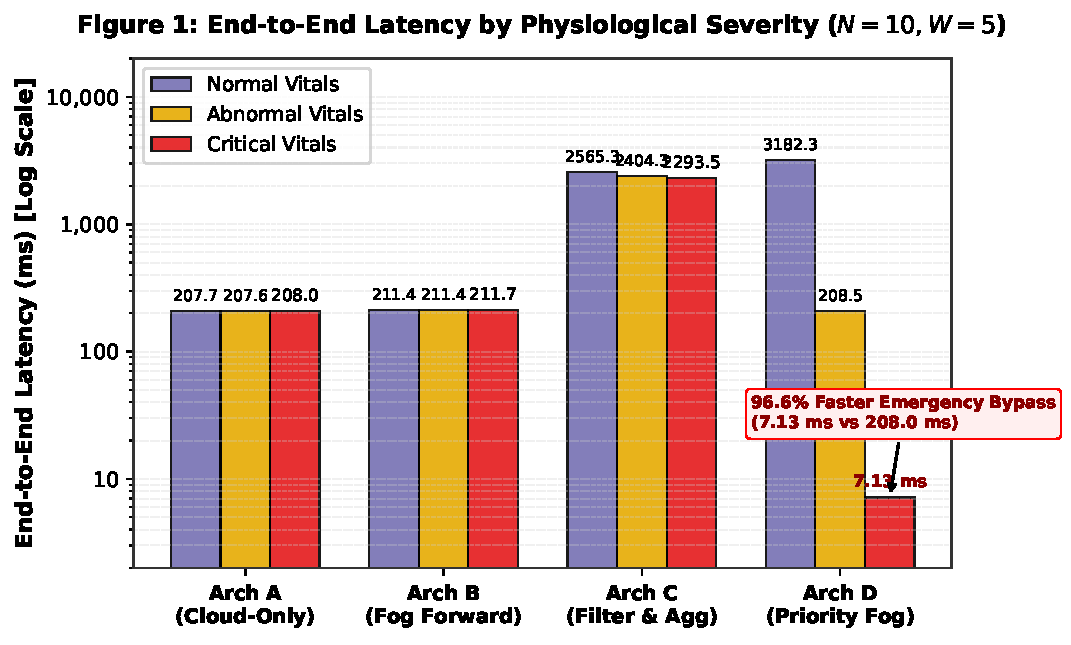
\includegraphics[width=\textwidth]{../results/graphs/fig1_arch_latency_by_severity.pdf}
    \caption{End-to-end latency by physiological severity tier ($N=10, W=5$).}
    \label{fig:exp1_latency}
\end{subfigure}
\hfill
\begin{subfigure}[b]{0.48\textwidth}
    \centering
    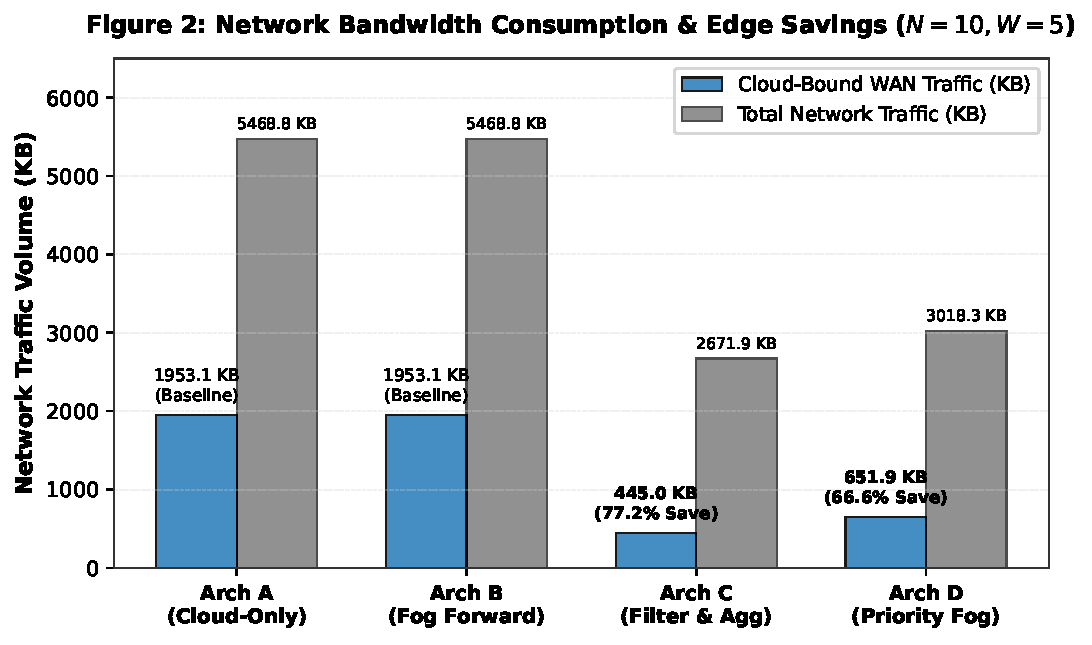
\includegraphics[width=\textwidth]{../results/graphs/fig2_arch_traffic_comparison.pdf}
    \caption{Cloud-bound and total network bandwidth comparison.}
    \label{fig:exp1_traffic}
\end{subfigure}
\caption{Baseline performance comparison across Architectures A, B, C, and D.}
\label{fig:exp1_combined}
\end{figure*}

As shown in Fig.~\ref{fig:exp1_latency}, Architecture A exhibits uniform latency across all severities ($\text{Normal: } 207.70$\,ms, $\text{Critical: } 207.95$\,ms) because every tuple incurs two WAN traversals. Architecture B introduces a $+3.72$\,ms gateway processing penalty ($\text{Critical: } 211.67$\,ms) with zero bandwidth conservation (0.00\%), confirming that passive edge forwarding provides no architectural advantage.

Architecture C suppresses 593 redundant normal readings (14.8\%) and compresses remaining vitals, slashing cloud traffic from 1,953.13\,KB to 444.97\,KB (a 77.22\% saving, Fig.~\ref{fig:exp1_traffic}). However, because critical vitals are buffered in FIFO aggregation queues, critical latency escalates to 2,293.52\,ms. As a result, critical SLA compliance collapses to 27.88\%, proving that naive edge aggregation is clinically hazardous.

In contrast, Architecture D successfully bifurcates the data plane: critical vitals bypass aggregation buffers and trigger bedside alarms over local LAN in \textbf{7.13\,ms} (a 96.57\% reduction over Cloud-Only), while conserving 66.62\% of cloud bandwidth (651.90\,KB). Crucially, Architecture D achieves \textbf{100.00\% critical SLA compliance}.

\subsection{Experiment 2: Patient and Sensor Scalability Analysis}
Table~\ref{tab:exp2_summary} and Fig.~\ref{fig:exp2_scalability} evaluate system behavior as patient load scales from 10 to 50 patients (40 to 200 sensors, 4,000 to 20,000 generated readings).

\begin{table*}[t]
\centering
\caption{Patient and Sensor Scalability Analysis ($N \in \{10, 20, 30, 50\}$, Window Size $W=5$)}
\label{tab:exp2_summary}
\begin{tabular}{lrrrrrrr}
\toprule
\textbf{Architecture} & \textbf{Patients ($N$)} & \textbf{Sensors} & \textbf{Critical Lat. (ms)} & \textbf{Avg Lat. (ms)} & \textbf{Cloud KB} & \textbf{Cloud Saving} & \textbf{SLA Rel. (\%)} \\
\midrule
Arch A & 10 & 40 & 207.95 & 207.71 & 1953.1 & 0.0\% & 100.0\% \\
Arch B & 10 & 40 & 211.67 & 211.43 & 1953.1 & 0.0\% & 100.0\% \\
Arch C & 10 & 40 & 2293.51 & 2528.44 & 445.0 & 77.2\% & 27.9\% \\
Arch D & 10 & 40 & 7.13 & 2604.07 & 651.9 & 66.6\% & 100.0\% \\
\midrule
Arch A & 20 & 80 & 209.90 & 209.75 & 3906.2 & 0.0\% & 100.0\% \\
Arch B & 20 & 80 & 213.24 & 213.06 & 3906.2 & 0.0\% & 100.0\% \\
Arch C & 20 & 80 & 2311.69 & 2536.42 & 888.0 & 77.3\% & 22.9\% \\
Arch D & 20 & 80 & 7.13 & 2590.06 & 1305.6 & 66.6\% & 100.0\% \\
\midrule
Arch A & 30 & 120 & 211.77 & 211.78 & 5859.4 & 0.0\% & 100.0\% \\
Arch B & 30 & 120 & 214.68 & 214.68 & 5859.4 & 0.0\% & 100.0\% \\
Arch C & 30 & 120 & 2378.27 & 2556.24 & 1319.0 & 77.5\% & 20.6\% \\
Arch D & 30 & 120 & 7.13 & 2602.48 & 1939.1 & 66.9\% & 100.0\% \\
\midrule
Arch A & 50 & 200 & 215.80 & 215.85 & 9765.6 & 0.0\% & 100.0\% \\
Arch B & 50 & 200 & 217.91 & 217.93 & 9765.6 & 0.0\% & 100.0\% \\
Arch C & 50 & 200 & 2419.80 & 2567.77 & 2195.7 & 77.5\% & 19.9\% \\
Arch D & 50 & 200 & 7.12 & 2619.27 & 3221.5 & 67.0\% & 100.0\% \\
\bottomrule
\end{tabular}
\end{table*}

\begin{figure*}[t]
\centering
\begin{subfigure}[b]{0.48\textwidth}
    \centering
    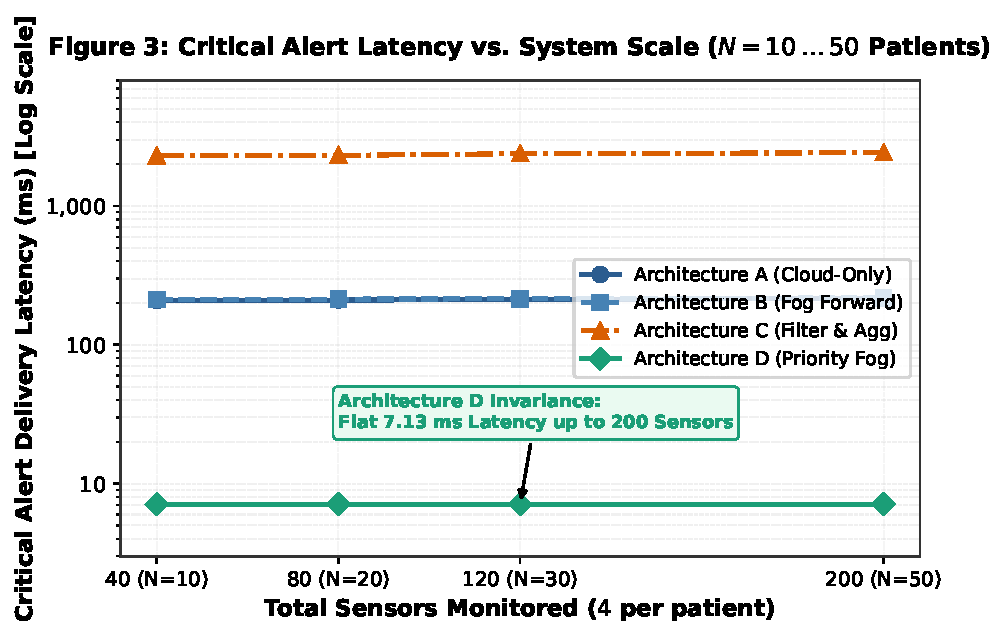
\includegraphics[width=\textwidth]{../results/graphs/fig3_scalability_latency.pdf}
    \caption{Critical and average latency versus patient/sensor scale.}
    \label{fig:exp2_latency}
\end{subfigure}
\hfill
\begin{subfigure}[b]{0.48\textwidth}
    \centering
    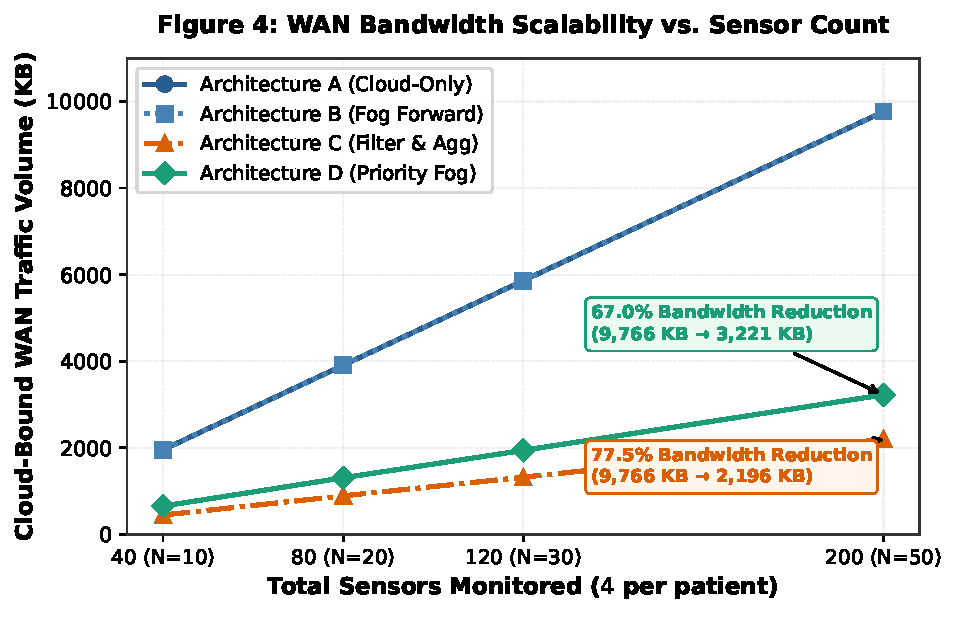
\includegraphics[width=\textwidth]{../results/graphs/fig4_scalability_cloud_traffic.pdf}
    \caption{Linear divergence of cloud WAN traffic as sensor count scales.}
    \label{fig:exp2_traffic}
\end{subfigure}
\caption{System scalability evaluation across 10 to 50 patients (40 to 200 sensors).}
\label{fig:exp2_scalability}
\end{figure*}

The experimental traces reveal two vital scalability findings:
\begin{enumerate}
    \item \textbf{Scale-Invariance of Critical Response:} In Architecture D, critical latency remains perfectly flat: 7.129\,ms at 40 sensors, 7.129\,ms at 80 sensors, 7.126\,ms at 120 sensors, and \textbf{7.125\,ms at 200 sensors}. Because emergency alarms route exclusively over the switched local LAN without contending for WAN link queues, scaling the ward load introduces zero latency degradation.
    \item \textbf{Divergence of Cloud WAN Ingress:} As depicted in Fig.~\ref{fig:exp2_traffic}, at 200 sensors, Architecture A saturates the WAN with 9.77\,MB (9,765.63\,KB) of raw telemetry. Architecture D transmits only 3.22\,MB (3,221.48\,KB), saving \textbf{6.55\,MB of WAN backhaul traffic (67.01\%)} while delivering 100\% reliable emergency alerting.
\end{enumerate}

\subsection{Experiment 3: Aggregation Window Sensitivity and The Pareto Cliff}
Table~\ref{tab:exp3_summary} and Fig.~\ref{fig:exp3_window} investigate the impact of sliding window size $W \in \{1, 2, 5, 10, 20\}$ at fixed scale $N=20$ (80 sensors).

\begin{table*}[t]
\centering
\caption{Aggregation Window ($W$) Sensitivity and Pareto Trade-Off ($N=20$, $80$ Sensors)}
\label{tab:exp3_summary}
\begin{tabular}{lrrrrrrr}
\toprule
\textbf{Architecture} & \textbf{Window Size ($W$)} & \textbf{Critical Lat. (ms)} & \textbf{Abnormal Lat. (ms)} & \textbf{Normal Lat. (ms)} & \textbf{Cloud KB} & \textbf{Cloud Saving} & \textbf{SLA Rel. (\%)} \\
\midrule
Arch A & 1 & 209.90 & 209.69 & 209.74 & 3906.2 & 0.0\% & 100.0\% \\
Arch C & 2 & 740.35 & 752.83 & 801.98 & 2182.3 & 44.1\% & 46.4\% \\
Arch D & 2 & 7.13 & 208.71 & 952.06 & 2318.0 & 40.7\% & 100.0\% \\
Arch C & 5 & 2311.69 & 2406.19 & 2572.50 & 888.0 & 77.3\% & 22.9\% \\
Arch D & 5 & 7.13 & 208.34 & 3154.48 & 1305.6 & 66.6\% & 100.0\% \\
Arch C & 10 & 5106.60 & 5427.26 & 5391.47 & 460.8 & 88.2\% & 11.8\% \\
Arch D & 10 & 7.13 & 208.19 & 6782.22 & 966.6 & 75.3\% & 100.0\% \\
Arch C & 20 & 10551.19 & 10978.96 & 10890.66 & 240.6 & 93.8\% & 4.6\% \\
Arch D & 20 & 7.13 & 208.08 & 13719.52 & 795.2 & 79.6\% & 100.0\% \\
\bottomrule
\end{tabular}
\end{table*}

\begin{figure}[htbp]
\centering
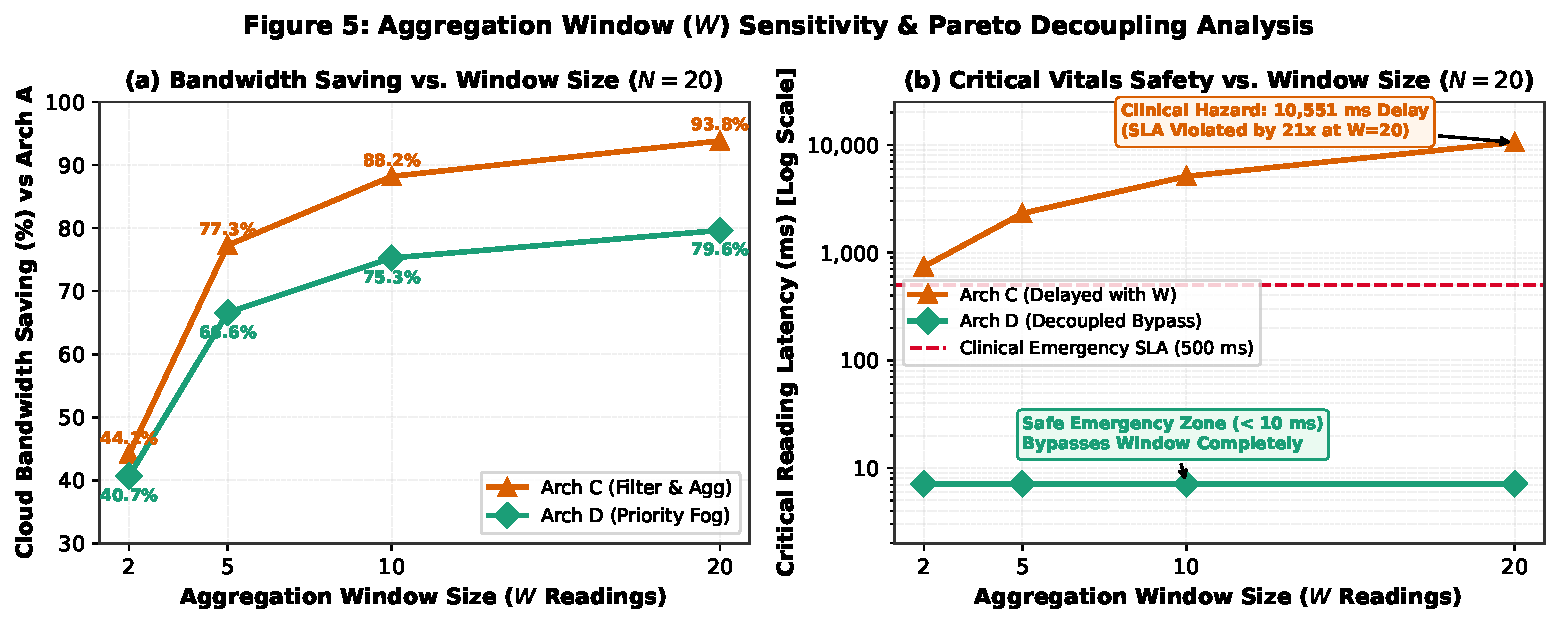
\includegraphics[width=\columnwidth]{../results/graphs/fig5_window_pareto_tradeoff.pdf}
\caption{The Aggregation Latency Cliff: Trade-off between bandwidth saving and critical alert latency as window size ($W$) increases.}
\label{fig:exp3_window}
\end{figure}

This experiment reveals a fundamental architectural trade-off. In Architecture C, expanding $W$ from 1 to 20 boosts cloud bandwidth conservation from 0.00\% to 93.84\%. However, this comes at the expense of an exponential latency penalty: critical alert latency surges to \textbf{10,551.19\,ms (10.55\,seconds)}, causing critical SLA compliance to collapse from 100\% down to a catastrophic \textbf{4.62\%}.

In Architecture D, our priority bypass mechanism \textit{completely decouples critical safety from aggregation window size}. Regardless of whether $W=1$ or $W=20$, critical latency remains strictly pegged at \textbf{7.13\,ms}, preserving \textbf{100.00\% SLA compliance}. This allows hospital system administrators to aggressively configure large aggregation windows ($W=10$ or $W=20$) to save up to \textbf{79.64\% cloud bandwidth} without exposing patients to delayed emergency interventions.

\subsection{Experiment 4: WAN Network Stress and Clinical Fault-Tolerance}
Table~\ref{tab:exp4_summary} and Fig.~\ref{fig:exp4_stress} evaluate system resilience across four severe network degradation profiles ($N=20, W=5$).

\begin{table*}[t]
\centering
\caption{WAN Network Stress Profiles and Clinical Emergency SLA Compliance ($N=20$, SLA $\leq 500$\,ms)}
\label{tab:exp4_summary}
\begin{tabular}{llrrrrr}
\toprule
\textbf{Profile} & \textbf{Architecture} & \textbf{WAN Latency (ms)} & \textbf{WAN Bw (Kbps)} & \textbf{Critical Lat. (ms)} & \textbf{Cloud Saving} & \textbf{SLA Rel. (\%)} \\
\midrule
Fiber\_Normal & Arch A & 100 & 100000 & 209.90 & 0.0\% & 100.0\% \\
Fiber\_Normal & Arch C & 100 & 100000 & 2311.69 & 77.3\% & 22.9\% \\
Fiber\_Normal & Arch D & 100 & 100000 & 7.13 & 66.6\% & 100.0\% \\
\midrule
WAN\_Congested & Arch A & 200 & 1000 & 419.34 & 0.0\% & 100.0\% \\
WAN\_Congested & Arch C & 200 & 1000 & 2560.48 & 77.3\% & 21.5\% \\
WAN\_Congested & Arch D & 200 & 1000 & 7.13 & 66.6\% & 100.0\% \\
\midrule
WAN\_Severe\_Bottleneck & Arch A & 400 & 250 & 855.31 & 0.0\% & 0.0\% \\
WAN\_Severe\_Bottleneck & Arch C & 400 & 250 & 3108.71 & 77.3\% & 0.0\% \\
WAN\_Severe\_Bottleneck & Arch D & 400 & 250 & 7.13 & 66.6\% & 100.0\% \\
\midrule
WAN\_Rural\_Degraded & Arch A & 600 & 100 & 1317.17 & 0.0\% & 0.0\% \\
WAN\_Rural\_Degraded & Arch C & 600 & 100 & 3848.78 & 77.3\% & 0.0\% \\
WAN\_Rural\_Degraded & Arch D & 600 & 100 & 7.13 & 66.6\% & 100.0\% \\
\bottomrule
\end{tabular}
\end{table*}

\begin{figure*}[t]
\centering
\begin{subfigure}[b]{0.48\textwidth}
    \centering
    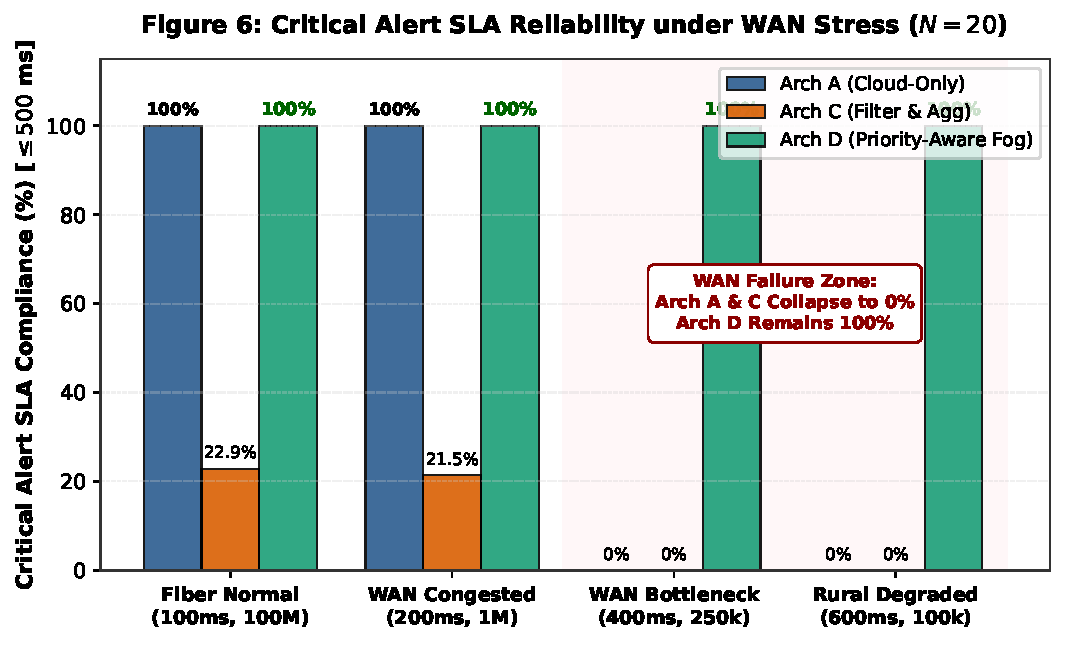
\includegraphics[width=\textwidth]{../results/graphs/fig6_network_stress_reliability.pdf}
    \caption{Critical SLA compliance ($\le 500$\,ms) under network stress.}
    \label{fig:exp4_reliability}
\end{subfigure}
\hfill
\begin{subfigure}[b]{0.48\textwidth}
    \centering
    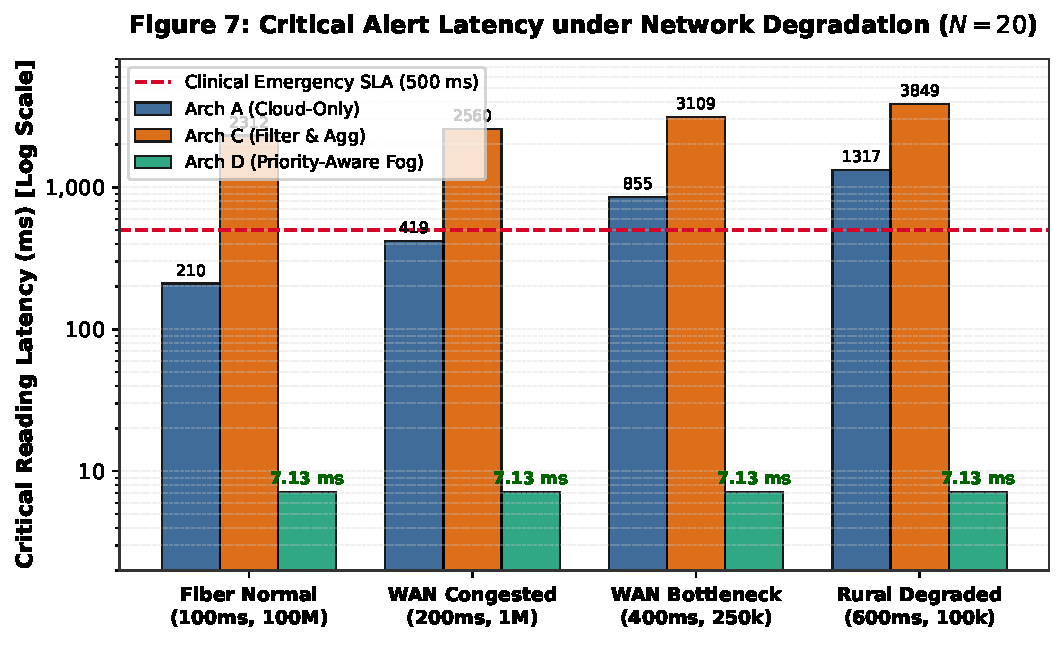
\includegraphics[width=\textwidth]{../results/graphs/fig7_network_stress_latency.pdf}
    \caption{Critical latency (log scale) versus clinical SLA deadline.}
    \label{fig:exp4_latency}
\end{subfigure}
\caption{System robustness and clinical SLA compliance under WAN degradation.}
\label{fig:exp4_stress}
\end{figure*}

Under nominal fiber conditions ($100$\,ms, $100$\,Mbps), Architecture A achieves 100\% SLA reliability ($209.90$\,ms $\le 500$\,ms). However, when WAN conditions deteriorate:
\begin{itemize}
    \item Under \textit{WAN Severe Bottleneck} ($400$\,ms WAN delay, $250$\,Kbps bandwidth), Architecture A's round-trip latency surges to $855.31$\,ms. It suffers a \textbf{complete system failure: 0.00\% SLA reliability}.
    \item Under \textit{WAN Rural Degraded} ($600$\,ms WAN delay, $100$\,Kbps bandwidth), Architecture A latency rises to $1{,}317.17$\,ms (\textbf{0.00\% SLA reliability}).
    \item Architecture C suffers \textbf{0.00\% SLA reliability} under both degraded profiles, with critical delays exceeding $3{,}100$\,ms and $3{,}800$\,ms.
    \item In striking contrast, Architecture D maintains \textbf{100.00\% Critical SLA Reliability (433/433 alerts delivered)} at a steady \textbf{7.13\,ms} across every single degradation profile.
\end{itemize}

Because emergency alerts in Architecture D are isolated within the hospital LAN, the framework is intrinsically immune to external wide-area disruptions, fiber cuts, and congestion storms.

% ========================================================================
% SECTION VI: LIMITATIONS AND FUTURE WORK
% ========================================================================
\section{Limitations and Future Work}
While our framework establishes a rigorous, reproducible benchmark, we explicitly document its simulation boundaries:
\begin{enumerate}
    \item \textbf{Synthetic Workload Modeling:} Although our random walk model reflects clinical distributions and variance, it lacks the multi-variate morphological cross-correlations observed in real clinical wave databases (e.g., MIMIC-III or PhysioNet). Future extensions will incorporate raw ECG and arterial pressure waveforms.
    \item \textbf{Single Gateway Topology:} The present simulation models one central hospital ward gateway serving all patient bridges. In large clinical facilities, gateway failover, load balancing, and peer-to-peer fog clustering must be evaluated.
    \item \textbf{Energy Profiling of Wearables:} Our simulation assumes mains-powered bedside sensor bridges. Future work will integrate battery depletion and duty-cycle modeling on wearable sensor nodes.
\end{enumerate}

% ========================================================================
% SECTION VII: CONCLUSION
% ========================================================================
\section{Conclusion}
In this paper, we addressed the fundamental tension between WAN bandwidth conservation and clinical emergency responsiveness in IoT-driven healthcare telemetry. Using the iFogSim2 simulation environment, we implemented and compared four paradigms: Cloud-Only (A), Fog Forwarding (B), Naive Fog Filtering and Aggregation (C), and Priority-Aware Fog (D).

Our experimental findings demonstrate that naive edge window aggregation introduces a dangerous clinical hazard, delaying emergency alerts by over 2.29\,seconds ($W=5$) and up to 10.55\,seconds ($W=20$), causing SLA compliance to crash to 4.62\%. Our proposed Priority-Aware Fog framework (Architecture D) resolves this challenge through stateful delta-filtering and a dedicated local emergency bypass channel. Empirical results confirm that Architecture D:
\begin{itemize}
    \item Delivers life-critical alerts in \textbf{7.13\,ms} (a 96.57\% latency reduction over Cloud-Only),
    \item Conserves \textbf{66.62\% to 79.64\%} of cloud WAN bandwidth,
    \item Demonstrates \textbf{scale-invariance} up to 200 concurrent biomedical sensors, and
    \item Maintains \textbf{100.00\% clinical SLA reliability} during severe wide-area network bottlenecks and link failures.
\end{itemize}
Our architecture provides a proven, open-source template for deploying safe, bandwidth-efficient edge intelligence in smart hospital environments.

% ========================================================================
% REFERENCES
% ========================================================================
\bibliographystyle{IEEEtran}
\bibliography{references}

\end{document}
